\chapter{Details of A Solution}
\section{CERT Secure Coding Standard }
The CERT Secure Coding Standard provides rules and recommendations (collectively called guidelines) for secure coding in the particular programming language. The goal of these rules and recommendations is to develop safe, reliable, and secure systems. Conformance to the coding rules defined in this standard are necessary (but not sufficient) to ensure the safety, reliability, and security of software systems developed in the programming language. 
Currently CERT developed coding standard for Android, C, C++, Java, Perl.

\subsection{Issues Not Addressed}
The following issues are not addressed by this standard:
\begin{itemize}
	\item \textbf{Design and Architecture.} Design level vulnerabilities are one of the dangerous ones. There are many standards to avoid design level vulnerabilities. This standard assumes that the product is free of design-level vulnerabilities
	
	\item \textbf{Coding Style.} Coding style issues are subjective; it has proven impossible to develop a
	consensus on appropriate style rules. This standard doesn't provide any coding styles.The easiest way to consistently apply a coding style is with the
	use of a code formatting tool. 
	
	\item \textbf{Tools.} SEI-CERT team didn't recommend  a particular vendors or
	tools.The developer can choose tools to enforce these rules.
	\item \textbf{ Controversial Rules} In general, the CERT secure coding standards try to avoid the
	inclusion of controversial rules that lack a broad consensus.
\end{itemize}
\subsection{Identifiers}
Each rule has a unique identifier, consisting of three parts:
\begin{itemize}
	\item \textbf{A three-letter mnemonic}, representing the section of the standard, is used to group similar rules and make them easier to find.
	\textit{eg: PRE: for preprocessor}
	\item \textbf{A two-digit numeric value} in the range of 00 to 99, which ensures each rule has a unique identifier.
	\textit{eg: PRE30}
	\item \textbf{The letter J/C}, which indicates that this is a Java language/C language rule and is included to prevent ambiguity with similar rules in CERT secure coding standards for other languages.
	\textit{eg: PRE30-C}
	Finally, the rule looks like,
	\textit{eg: PRE30-C - Do not create a universal character name through concatenation}
\end{itemize}

\subsection{Priority and Levels}
Each rule has an assigned priority. Priorities are assigned using a metric based on Failure
Mode, Effects, and Criticality Analysis. Three values are assigned
for each rule on a scale of 1 to 3 for
\newline
\newline
\textbf{ Severity} How serious are the consequences of the rule being ignored:
\begin{itemize}
	\item 1 = low  
	The effect is denial-of-service attack, abnormal termination 
	\item 2 = medium 
	The effect is data integrity violation, unintentional information disclosure)
	\item 3 = high 
	The effect is run arbitrary code, privilege escalation)
\end{itemize}

\textbf{Likelihood} The probability that a flaw introduced by violating the rule could lead to an exploitable vulnerability:
\begin{itemize}
	\item 1 = unlikely
	\item 2 = probable
	\item 3 = likely
\end{itemize}

\textbf{Remediation cost} How expensive is it to remediate existing code to comply with the rule:
\begin{itemize}
	\item 1 = high
	The effect is manual detection and correction.
	\item 2 = medium
	The effect is automatic detection and manual correction.
	\item 3 = low
	The effect is automatic detection and correction.
\end{itemize}
The three values are multiplied together for each rule. This product provides a measure to prioritize the rules. These products range from 1 to 27. Rules with a priority in the range of 1 to 4 are level 3 rules, 6 to 9 are level 2, and 12 to 27
are level 1. As a result, it is possible to claim level 1, level 2, or complete compliance (level 3)
with a standard by implementing all rules in a level, as shown in Figure \ref{fig:1}\cite{cert-c}
\begin{figure}[H]
	
	
	\centering
	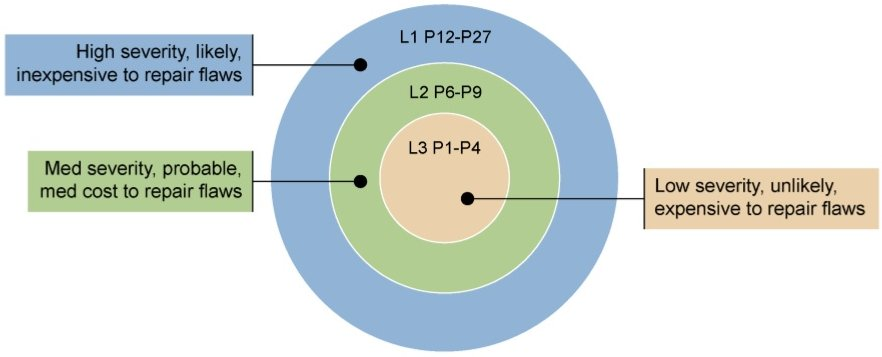
\includegraphics[width=.9\linewidth]{Figures/lev}
	\caption{Levels and priority ranges}	 
	\label{fig:1}
	
\end{figure}

\subsection{Rules and Recommendations}
Rules are normalized ones. It is mandatory to follow rules.Rules must meet the following criteria:
\begin{enumerate}
	
	\item Violation of the guideline is likely to result in a defect that may adversely affect the safety, reliability, or security of a system
	\item The guideline does not rely on source code annotations or assumptions.
	Rules are identified by the label rule.
\end{enumerate}
Recommendations are not normalized. Recommendations are suggestions for improving code quality.It is not mandatory to follow recommendations Guidelines are defined to be recommendations when all of the following conditions are met:
\begin{enumerate}
	
	\item Application of a guideline is likely to improve the safety, reliability, or security of software systems.
	\item One or more of the requirements necessary for a guideline to be considered a rule cannot be met.
\end{enumerate}	
Recommendations are identified by the label recommendation.

\section{CERT Android Secure Coding Standard}
 The Android standards are classified into C, Java, Android only rules. Out of this three Android only rules are under development stage, so these  are incomplete or contain errors. There are twenty eight rules listed in CERT website related to Android, but these are not matured. They haven't published any report or book form as official releases. But some of the standardized and officially released CERT C and Java secure coding rules are applicable to developing Android applications. There are 17 Android C rules and 10 recommendations. In the case of Android Java 160 rules and 46 recommendations are available. Table \ref{tab:andrc} and table \ref{tab:andrjava} gives an idea about Android C and Java rules.
 \\
 \begin{table}[h!]
 	\centering
 	
 	\label{tab:andrc}
 	
 	\begin{tabular}{|l|c|c|c|}
 		\hline
 		\textbf{Rule Id} & \textbf{Name} & \textbf{Rules} & \textbf{Recommendations}\\
 		
 		\hline
 		01 & Preprocessor (PRE) & - & -\\
 		\hline
 		
 		02 & Declarations and Initialization (DCL) & 01 & -\\
 		\hline
 		
 		03 & Expressions (EXP) & 01 & -\\
 		\hline
 		
 		04 & Integers (INT) & 01 & -\\
 		\hline
 		
 		05 & Floating Point (FLP) & 03 & 04\\
 		\hline
 		
 		06 & Arrays (ARR) & - & -\\
 		\hline
 		
 		07 & Characters and Strings (STR) & 02 & 01\\
 		\hline
 		
 		08 & Memory Management (MEM) & 01 & -\\
 		\hline
 		
 		09 & Input Output (FIO) & 03 & -\\
 		\hline
 		
 		10 & Environment (ENV) & - & -\\
 		\hline
 		
 		11 & Signals (SIG) & 04 & 03\\
 		\hline
 		
 		12 & Error Handling (ERR) & - & -\\
 		\hline
 		
 		13 & Application Programming Interfaces (API) & - & 02\\
 		\hline
 		
 		14 & Concurrency (CON) & - & -\\
 		\hline
 		
 		48 & Miscellaneous (MSC) & 01 & -\\
 		\hline
 		
 		50 & POSIX (POS) & - & -\\
 		\hline
 		
 	\end{tabular}
 	\caption{Categories in the CERT Android C secure coding standard}
 \end{table}
 
 
 
 \begin{table}[h!]
 	\centering
 	
 	\label{tab:andrjava}
 	\begin{tabular}{|l|c|c|c|}
 		\hline
 		\textbf{Rule Id} & \textbf{Name} & \textbf{Rules} & \textbf{Recommendations}\\
 		\hline
 		
 		00 & Input Validation and Data Sanitization (IDS) & 14 & 6\\
 		\hline
 		
 		01 & Declarations and Initialization (DCL) & 03 & -\\
 		\hline
 		02 & Expressions (EXP) & 07 & 02\\
 		\hline
 		03 & Numeric Types and Operations (NUM) & 14 & 04\\
 		\hline
 		04 & Characters and Strings (STR) & - & -\\
 		\hline
 		05 & Object Orientation (OBJ) & 12 & -\\
 		\hline
 		06 & Methods (MET) & 13 & 03\\
 		\hline
 		07 & Exceptional Behavior (ERR) & 10 & 01\\
 		\hline
 		08 & Visibility and Atomicity (VNA) & 06 & -\\
 		\hline
 		09 & Locking (LCK) & 12 & 3\\
 		\hline
 		10 & Thread APIs (THI) & 06 & 05\\
 		\hline
 		11 & Thread Pools (TPS) & 05 & 05\\
 		\hline
 		12 & Thread-Safety Miscellaneous (TSM) & 4 & 03\\
 		\hline
 		13 & Input Output (FIO) & 16 & 07\\
 		\hline
 		14 & Serialization (SER) & 12 & -\\
 		\hline
 		15 & Platform Security (SEC) & 08 & 04\\
 		\hline
 		16 & Runtime Environment (ENV) & 06 & 02\\
 		\hline
 		17 & Java Native Interface (JNI) & 04 & -\\
 		\hline
 		49 & Miscellaneous (MSC) & 8 & 01\\
 		\hline
 		
 	\end{tabular}
 	\caption{Categories in the CERT Android Java secure coding standard}
 \end{table}
 

 
The proposed system will verify Android Java rules only. So the solutions of CERT rules will deal only with Android Java rules.

\section{Solution for CERT rules}

\subsection{DCL00-J. Prevent class initialization cycles  (Intraclass Cycle)}

Initialization of a class consists of executing its static initializers and the initializers for static fields (class variables) declared in the class. Therefore, the presence of a static field triggers the initialization of a class. However, the initializer of a static field could depend on the initialization of another class, possibly creating an initialization cycle\cite{dcl00j}. There are two types of class initialization cycle problem, Intraclass and interclass. In intraclass the cycle will present within a class. In inter-class, the cycle will present between two class. 

The vulnerability  happened because the constructor invocation is done before completing the initialization of the variables. The solution is, do the object creation after the complete variable initialization. 


\subsubsection{Non-compliant Code Example (Intraclass Cycle)}
\begin{lstlisting}
public class RollNo {
private final int idNumber;
private static final RollNo r= new RollNo();
private static final int seed = (int) (Math.random() * 100);  

public RollNo() {
idNumber = seed - 10;  
}

public static void main(String[] args) {
System.out.println("Your unique id is: " + r.idNumber);
}
}
\end{lstlisting}
In the non-compliant code, there is a static final variable initialization after class object creation. 
 
\subsubsection{Compliant Code Example (Intraclass Cycle)}
 
\begin{lstlisting}
public class RollNo {
private final int idNumber;
private static final int seed = (int) (Math.random() * 100);  
private static final RollNo r= new RollNo();

public RollNo() {
idNumber = seed - 10; 
}

public static void main(String[] args) {
System.out.println("Your unique id is: " + r.idNumber);
}
}
\end{lstlisting}
 

In the  compliant code, the static final variable initialization done before class object creation.


\subsubsection{Applicability of the rule}
If there is an object creation (Constructor invocation) between some static final variable declaration then DCL001-J Intraclass Cycle vulnerability may present. The given algorithm will check the applicability of the rule.

\textbf{Algorithm}

\begin{lstlisting}
	
1. Read .java file (sb)
2. str = sb.toString(); // Convert to string
3. parser.setSource(str.toCharArray()); // Parse(str)
4.CompilationUnit cu = (CompilationUnit) parser.createAST(null); // Set CompilationUnit
5.cu.accept(new MyVisitor(cu,str));
6. In MyVisitor class
	1. For each class visit(TypeDeclaration node) // Visit type declaration with node variable
	2. this.Classname=node.getName()toString(); //Get the class name from it
	3. For each Field visit(FieldDeclaration node) // Visit FieldDeclaration node
		1. For each visit(VariableDeclarationFragment fd)
		2. VarList.add(fd.getName().toString()); //Save all variables to a public list VarList
		3.  LineList.add(cu.getLineNumber(fd.getStartPosition()));  // Save position to a public list LineList
		4. For each visit(MethodDeclaration md)
			1. String s=fd.getRightHandSide().toString();
			2. for(int i=0;i<VarList.size();i++)
			if(s.contains(VarList.get(i)))  // Check static variable present in VarList
				1.if(LineList.get(i)>0&&Clno>0){ // Check variable declaration and constructor initialization with "Static" keyword is present
					1.if(LineList.get(i)>Clno)//  Check variable declaration is after constructor initialization 
						1. If yes return "DCL00-J Vulnerability is there"
\end{lstlisting}
	 
\subsubsection{Semi-algorithmically explanation}
/* Yet to finish */
\subsubsection{Semi-automatic quick fixes} 
 /* Yet to finish */
\subsection{DCL01-J. Do not reuse public identifiers from the Java Standard Library}
\subsubsection{Non-compliant Code Example}
\begin{lstlisting}
class StringBuffer {
private int val = 1;

public boolean isEmpty() {
if (val == 1) {   // Compares with 1 instead of 0
return true;
} else {
return false;
}
}
}
\end{lstlisting}
\subsubsection{Compliant Code Example}
/* Yet to finish */
\begin{lstlisting}
class MyStringBuffer {
private int val = 1;

public boolean isEmpty() {
if (val == 1) {   // Compares with 1 instead of 0
return true;
} else {
return false;
}
}
}
\end{lstlisting}
\subsubsection{Applicability of the rule}
/* Yet to finish */
\subsubsection{Semi-algorithmically explanation}
/* Yet to finish */
\subsubsection{Semi-automatic quick fixes} 
/* Yet to finish */
 


% -eof-


% -eof-
